David Rohrbaugh

2014-12-5

Encoders, Wiring, and the Launching Mechanism

\begin{tabular}{|p{5cm}|p{5cm}|}
 \hline
 I did a little bit of everything this week. I put encoders on the two drive motors, worked with everyone else on the wiring another day, and helped Alex with the new plastic launching mechanism.
 &
 The encoders have not been tested yet, as the wiring is still being figured out, but they should work. I believe that the wiring is nearing completion. Our robot is starting to come together, as even with a flimsier cardboard launching mechanism it can fling a ball to the required height. Eventually, this fling will be directed into the goal with another mechanism. We replaced the cardboard with plastic.
 \\
 \hline
\end{tabular}

\medskip

This is a graphical representation of our overall plan for getting balls into goals:

\begin{center}
 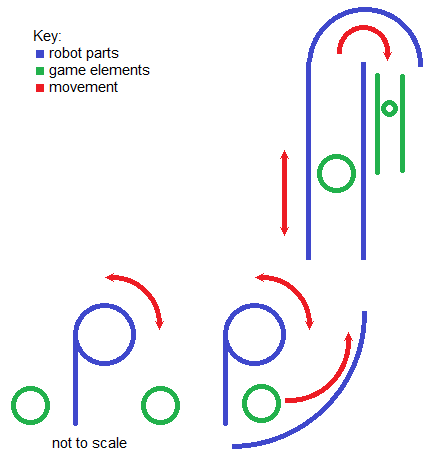
\includegraphics{./Entries/Images/scoring_design.png}
\end{center}

The basic idea goes something like this: the first spinner collects balls, the second spinner launches the balls into the tube, which redirects them into the goal.
The redirect tube has yet to be implemented, but we have some materials available that may be suitable, e.g. metal ducts.
